\documentclass[finnish, svgnames]{beamer}

\definecolor{sciorange}{RGB}{252,163,17}
\definecolor{unigray}{RGB}{140,140,140}
\mode<presentation>
 {
 \usetheme{Berlin}
 \usefonttheme{professionalfonts}
 \setbeamertemplate{headline}{}
 \setbeamertemplate{itemize item}{\color{sciorange}$\blacksquare$}
 \setbeamertemplate{itemize subitem}{\color{unigray}\scalebox{0.759383838348}{$\blacksquare$}}
 \setbeamercolor*{palette primary}{use=structure,fg=white,bg=sciorange}
 \setbeamercolor*{palette secondary}{use=structure,fg=white,bg=unigray}
 \setbeamercolor*{palette tertiary}{use=structure,fg=white,bg=unigray}
 \setbeamercolor*{palette quartenary}{use=structure,fg=white,bg=unigray}
 \setbeamercolor{block title}{fg=sciorange}
 \setbeamercolor{local structure}{fg=sciorange}
 \setbeamercolor{section in toc}{fg=black,bg=black}
 \usebackgroundtemplate{%
\tikz[overlay,remember picture] \node[opacity=0.2, at=(current page.center)] {
   
\includegraphics[height=2in]{flame}};
}
 }

\usepackage[utf8]{inputenc}
%\usepackage[T1]{fontenc}
%\usepackage{lmodern}
%\usepackage{microtype}
%\usepackage{amsfonts,amsmath,amssymb,amsthm,booktabs,color,enumitem,graphicx}
%\usepackage[pdftex,hidelinks]{hyperref}
%\usepackage[dvipsnames]{xcolor}
%\usepackage{soul}
%\usepackage{algorithm}
%\usepackage{algorithmic}
%\usepackage[algo2e]{algorithm2e}
%\usepackage{float}
\usepackage{tikz}
\usetikzlibrary{arrows,automata}
%\usetikzlibrary{arrows,automata}
\usepackage{amsmath}
\usepackage{soul}
\usepackage{color}
\usepackage{lmodern}

\begin{document}
    \title[] % (optional, only for long titles)
{Maksimivirtauksen löytäminen verkossa}
\subtitle{Tiralabra}
\author[Chang Rajani] % (optional, for multiple authors)
{Chang Rajani}
\institute[Helsingin Yliopisto] % (optional)
{

  Tietojenkäsittelytieteen laitos\\
  Helsingin Yliopisto
  %\and
  %\inst{2}%
  %Institute of Theoretical Philosophy\\
  %University There
}
\date[2016] % (optional)
{Tiralabran demo}
\subject{Computer Science}

\frame{\titlepage}

%\begin{frame}
%\frametitle{Esitelmän sisältö}
%\tableofcontents
%\end{frame}



\section{Ongelman määrittely}
\begin{frame}
  \frametitle{Ongelman määrittely: maksimivirtaus}
  \begin{itemize}
    \item Annettuna verkko, jossa on solmu $s$ josta on vain lähteviä kaaria, ja solmu $t$ johon on vain sisääntulevia kaaria
    \item Lisäksi verkossa on kaaripainoina kokonaislukuja jotka kuvastavat kapasiteettia (kuinka monta yksikköä virtausta saa kaaresta läpi)
    \item Voi kuvitella esim putkiverkostona missä putket ovat erikokoisia
  \end{itemize}

\end{frame}

  \begin{frame}
  \frametitle{Maksimivirtaus}
  \begin{figure}[t]
  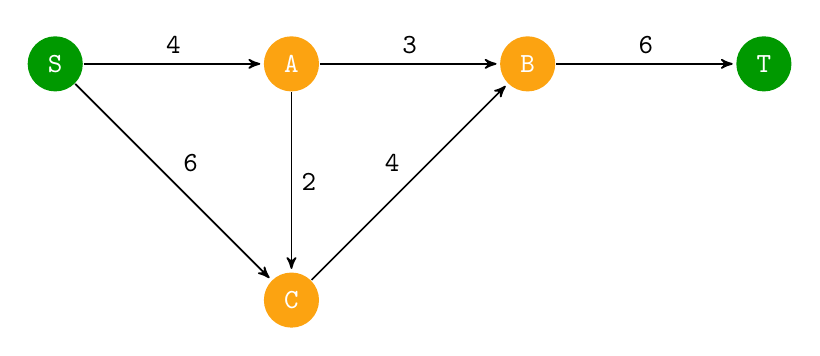
\begin{tikzpicture}[->,>=stealth',shorten >=1pt,auto,node distance=3cm,
                        semithick, font=\ttfamily]
      \tikzstyle{every state}=[fill=sciorange,draw=none,text=white,minimum size=0.7cm]

      \node[state,fill=black!40!green] (A) {S};
      \node[state] (B) [right of=A]  {A};
      \node[state] (C) [right of=B]  {B};
      \node[state] (D) [below of=B]  {C};
      \node[state,fill=black!40!green] (E) [right of=C]  {T};

      \path (A) edge node {4} (B)
                edge node {6} (D)
            (B) edge node {3} (C)
                edge node {2} (D)
            (C) edge node {6} (E)
            (D) edge node {4} (C)   ;

  \end{tikzpicture}
  %\caption{Merkkijonojen \{\texttt{anna, ann, bert, best}\} trie. Kaksoisympyröidyt solmut merkitsevät solmuja, joihin loppuva merkkijono löytyy joukosta.}
  \label{fig:verkko}
  \end{figure}
  \end{frame}

\begin{frame}
  \frametitle{Toteutetut algoritmit}
  \begin{itemize}
    \item Ford-Fulkerson
      \begin{itemize}
        \item Esiprosessoi verkon niin, että jokaista kaarta vastaa päinvastaiseen suuntaan oleva kaari
        \item 1. Löytää jonkun reitin verkossa syvyyshaulla
        \item 2. Kasvattaa virtausta reitin pienimmällä kapasiteetilla
        \item 3. Toistaa 1. kunnes ei löydy enää reittiä
        \item Löytää aina maksimivirtauksen $\mathcal{O}{(|V|*|f|)}$ ajassa, missä $|f|$ on maksimivirtaus
        \item Pahimmassa tapauksessa eksponentiaalinen
      \end{itemize}
  \end{itemize}

\end{frame}

\begin{frame}
\frametitle{Ford-Fulkerson verkossa}
\begin{figure}[t]
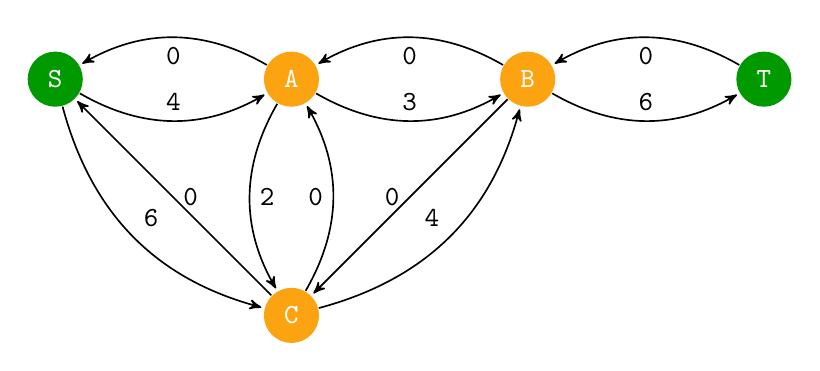
\begin{tikzpicture}[->,>=stealth',shorten >=1pt,auto,node distance=3cm,
                      semithick, font=\ttfamily]
    \tikzstyle{every state}=[fill=sciorange,draw=none,text=white,minimum size=0.7cm]

    \node[state,fill=black!40!green] (A) {S};
    \node[state] (B) [right of=A]  {A};
    \node[state] (C) [right of=B]  {B};
    \node[state] (D) [below of=B]  {C};
    \node[state,fill=black!40!green] (E) [right of=C]  {T};

    \path (A) edge[bend right] node {4} (B)
              edge[bend right] node {6} (D)
          (B) edge[bend right] node {3} (C)
              edge[bend right] node {0} (A)
              edge[bend right] node {2} (D)
          (C) edge[bend right] node {6} (E)
              edge node [left] {0} (D)
              edge[bend right] node {0} (B)
          (D) edge[bend right] node {4} (C)
              edge[bend right] node {0} (B)
              edge node [right] {0} (A)
          (E) edge[bend right] node {0} (C);

\end{tikzpicture}
%\caption{Merkkijonojen \{\texttt{anna, ann, bert, best}\} trie. Kaksoisympyröidyt solmut merkitsevät solmuja, joihin loppuva merkkijono löytyy joukosta.}
\label{fig:verkko}
\end{figure}
\end{frame}



\begin{frame}
  \frametitle{Toteutetut algoritmit}
  \begin{itemize}
    \item Edmonds-Karp
      \begin{itemize}
        \item Käyttää leveyshakua syvyyshaun sijasta
        \item Löytää siis lyhimmän reitin (eikä vaan jotain reittiä) joka kohdassa
        \item Aikavaativuus aina $\mathcal{O}{(|V|*|E|^2)}$
      \end{itemize}
  \end{itemize}
\end{frame}

\begin{frame}
  \frametitle{Toteutetut algoritmit}
  \begin{itemize}
    \item Scaling Flow
      \begin{itemize}
        \item Etsii ensin verkon suurimman kapasiteetin
        \item Yrittää sitten löytää reitin, joka kasvattaa virtausta vähintään tuon kapasiteetin verran
        \item Puolittaa etsittävän kapasiteetin koon
        \item Aikavaativuus aina $\mathcal{O}{(|E|^2 * log(|maxC|))}$, missä $maxC$ on verkon isoin kapasiteetti
      \end{itemize}
  \end{itemize}
\end{frame}

\section{Sovellukset}
\begin{frame}
  \frametitle{Sovellukset}
  \begin{itemize}
    \item Maksimiparitus kaksijakoisessa verkossa
    \item Minimileikkaus verkossa
    \item Suurin polkujoukko solmusta solmuun niin, että polut eivät mene päällekkäin
  \end{itemize}

\end{frame}

\end{document}
